\documentclass[a4paper, 12pt]{article} % тип документа

%%%Библиотеки
%\usepackage[warn]{mathtext}	
\usepackage[T2A]{fontenc}   %Кодировка
\usepackage[utf8]{inputenc} %Кодировка исходного текста
\usepackage[english, russian]{babel} %Локализация и переносы
\usepackage{caption}
\usepackage{gensymb}
%\usepackage{listings}
\usepackage{amsmath, amsfonts, amssymb, amsthm, mathtools}
%\usepackage[warn]{mathtext}
%\usepackage[mathscr]{eucal}
%\usepackage{wasysym}
\usepackage{graphicx} %Вставка картинок правильная
%\usepackage{pgfplots}
\usepackage{indentfirst}
% \usepackage{float}    %Плавающие картинки
\usepackage{wrapfig}  %Обтекание фигур (таблиц, картинок и прочего)
\usepackage{fancyhdr}  %Загрузим пакет
%\usepackage{lscape}
%\usepackage{xcolor}
%\usepackage[normalem]{ulem}
\usepackage{geometry}

\usepackage{titlesec}
\titlelabel{\thetitle.\quad}

\usepackage{hyperref}

\newgeometry{vmargin={20mm}, hmargin={25mm, 25mm}}
%%%Конец библиотек

%%%Настройка ссылок
\hypersetup
{
	colorlinks = true,
	linkcolor  = blue,
	filecolor  = magenta,
	urlcolor   = blue
}
%%%Конец настройки ссылок


%%%Настройка колонтитулы
\pagestyle{fancy}
\fancyhead{}
\fancyhead[L]{5.10.1}
\fancyhead[R]{Таранов Александр, группа Б01-206}
\fancyfoot[C]{\thepage}
%%%конец настройки колонтитулы


\begin{document}
	
	%%%Начало титульника
	\begin{titlepage}
		
		\newpage
		\begin{center}
			\normalsize Московский физико-технический институт \\(госудраственный университет)
		\end{center}
		
		\vspace{6em}
		
		\begin{center}
			\Large Лабораторная работа по общему курсу физики\\Квантовая физика
		\end{center}
		
		\vspace{1em}
		
		\begin{center}
			\Large \textbf{Исследование энергетического спектра $\beta$-частиц и определение их максимальной энергии при помощи магнитного спектрометра.}
		\end{center}
		
		\vspace{2em}
		
		\begin{center}
			\large Таранов Александр \\
			Группа Б01-206
		\end{center}
		
		\vspace{\fill}
		
	\end{titlepage}
	%%%Конец Титульника
	
	
	
	%%%Настройка оглавления и нумерации страниц
	\thispagestyle{empty}
	\newpage
	\tableofcontents
	\newpage
	\setcounter{page}{1}
	%%%Настройка оглавления и нумерации страниц

\section{Теоретическое введение}
	
\subsection{Основы бетта распада}
	
	$\beta$-распад -- явление самопроизвольного превращения ядер, в котором массовое число $A$ ядра сохраняется, а заряд изменяется на единицу. Ядра, подверженные $\beta$-распаду встречаются во всей области значений массового числа $A$. Диапазон энергий, высвобождаемых при $\beta$-распаде: $18 \text{ кэВ} \div 13.4 \text{ МэВ}$. Периоды полураспада лежат в пределах $10^{-6} \text{ с} \div 10^{18} \text{ лет}$.
	
	В данной работе изучается бета-минус-распад ($\beta^{-}$) ядра $^{137}$Cs:
	
	\begin{equation}
		^A_Z X \rightarrow ^{A}_{Z+1} X + e^{-} + \tilde{\nu}.
	\end{equation}
	В данном типе распада испускается электрон и антинейтрино.
	
	Поскольку масса ядра много больше массы электрона $A \cdot m_{p} \gg m_{e}$, энергия, уносимая ядром, очень мала. Однако, в эксперименте у электронов наблюдается сплошной спектр, который объясняется существованием антинейтрино, которое в состоянии унести оставшуюся энергию. Таким образом, электроны могут иметь любую энергию от нулевой до полной энергии, выделяемой при $\beta$-распаде $T_{max}$.
	
\subsection{Спектр $\beta$-электронов}
	
	Как было отмечено выше, спектр является непрерывным от нуля до $T_{max}$. $W$ -- спектральная плотность вероятности.
	
	Спектр $\beta$-электронов для разрешенных фермиевских переходов может быть рассчитан теоретически. В этом случае вероятность $\beta$-распада с заданными $p_e$ и $p_{\nu}$ пропорциональна статистическому весу. Поскольку энергия, уносимая ядром, мала, мы можем считать, что $T_e + E_{\nu} = T_{\beta} = T_{max}$. Тогда энергия и импульс нейтрино полностью определяются $p_e$.
	
	\begin{wrapfigure}[15]{r}{7.0cm}
		%              ^^ number of occupied rows
		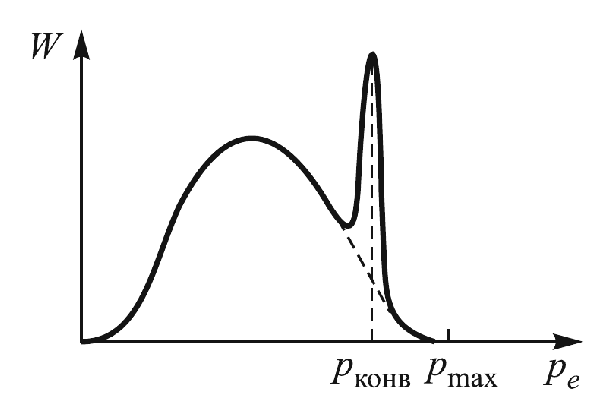
\includegraphics[scale=0.6]{res/spectrum.png}
		\caption{Спектр $\beta$-электронов.}
		\label{fig:spectrum}
		\vspace{0pt}
	\end{wrapfigure}
	
	Интервалу $(p_e; p_e + d p_e)$ соответствует фазовый объем $4 \pi p_e^2$. Аналогичный шаровой слой соответствует антинейтрино: $4 \pi p_{\nu}^2$. Тогда получаем:
	\begin{equation}
		W(p_e) dp_e \propto p_e^2 p_{\nu}^2 dp_e.
		\label{eq:probability}
	\end{equation}
	
	Выразим импульс антинейтрино:
	\begin{equation}
		p_{\nu} = E_{\nu} / c = \frac{T_{max} - T_e}{c}.
		\label{eq:impulse_nu}
	\end{equation}
	
	Подставляя \eqref{eq:impulse_nu} в \eqref{eq:probability} получаем:
	\begin{equation}
		W(p_e) dp_e \propto p_e^2 (\sqrt{p_{max}^2 + m_e^2 c^2} - \sqrt{p_e^2 + m_e^2 c^2})^2 dp_e.
	\end{equation}
	
	На спектре также наблюдается выраженный пик при $p_e = p_{\text{конв}}$. Этот пик называется конверсионным. При $\beta$-распаде ядро может оказаться возбужденным. Энергия возбуждения может быть излучена через $\gamma$-квант или передана электрону с внутренней оболочки атома. Эти электроны образуют монохроматический пик. Для $^{137}$Cs он расположен на энергии $T_{\text{к}} = 0.624$ МэВ.
	
\section{Методика эксперимента}
	
	\begin{figure}[h!]
		\centering
		\begin{minipage}{0.5\textwidth}
			\centering
			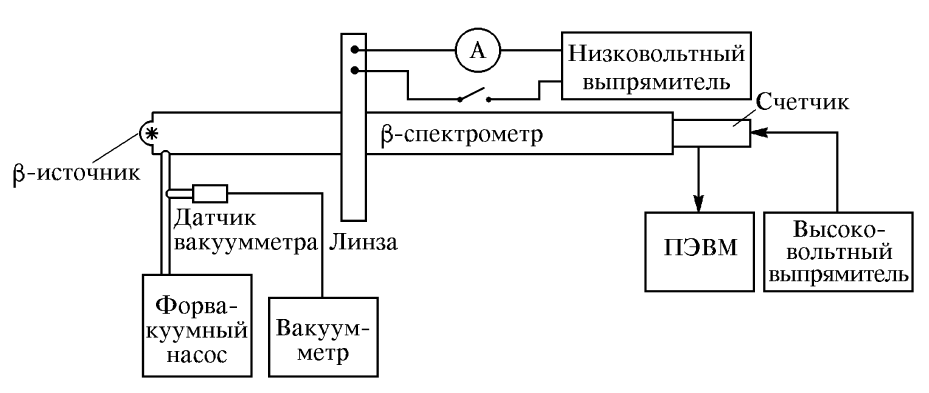
\includegraphics[width=1.0\linewidth]{res/setup.png}
		\end{minipage}%
		\begin{minipage}{0.5\textwidth}
			\centering
			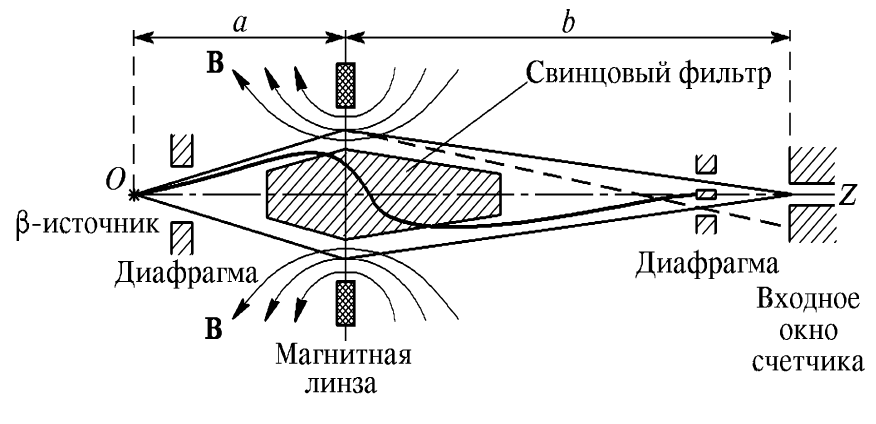
\includegraphics[width=1.0\linewidth]{res/scheme.png}
		\end{minipage}
		\caption{Схема установки для изучения $\beta$-распада.}
		\label{fig:setup_scheme}
	\end{figure}
	

	Для определения энергии $\beta$-частиц используется $\beta$-спектрометр с "короткой линзой". Электроны, испускаемые источником, попадают в магнитное поле катушки (магнитной линзы). В фокусе этой линзы расположен счетчик -- сцинтиллятор. Сигнал с сцинтиллятора попадает в ФЭУ, после чего с помощью АЦП сохраняется на компьютере.
	
	Для предотвращения попадания прямого $\gamma$-излучения и $\beta$-частиц устанавливается свинцовый фильтр. Магнитная линза имеет значительные сферические аберрации, для исключения их влияния необходимо устанавливать диафрагму.
	
	Для исключения рассеяния электронов в спектрометре с помощью форвакуумного насоса поддерживается давление $P \sim 0.1$ Торр.
	
	Для фокусного расстояния линзы можно показать, что:
	\begin{equation}
		\frac{1}{f} \propto \frac{I^2}{p_e^2},
		\label{eq:focus}
	\end{equation}
	где $I$ -- сила тока в линзе. При заданной силе тока в счетчик попадают электроны с импульсом $p_e \pm \Delta p_e / 2$. $\Delta p_e$ -- разрешающая способность спектрометра.
	
	Геометрия прибора не изменяется в ходе опыта, поэтому
	\begin{equation}
		p_e = kI,
	\end{equation}
	где $k$ -- константа прибора.
	
	Рассмотрим связь частоты регистрации частиц и спектральной плотности вероятности.
	$$N(p_e) = W(p_e) \cdot \Delta p_e.$$
	
	Исходя из \eqref{eq:focus} получим:
	$$ \Delta p_e = \frac{1}{2} \frac{\Delta f}{f} 	p_e.$$
	
	Тогда:
	\begin{equation}
		N(p_e) = C \cdot W(p_e) p_e
		\label{eq:fermi}
	\end{equation}
	
	\section{Результаты}
	
	Проведем измерения частоты регистрации частиц для токов в диапазоне $I = (0.0 \div 4.6)$ А. Каждое измерение проводится в течение 60 секунд. Для учета фона вычтем из $N$ значение $N_0$ при $I = 0$ А.
	
	\begin{figure}[h!]
		\centering
		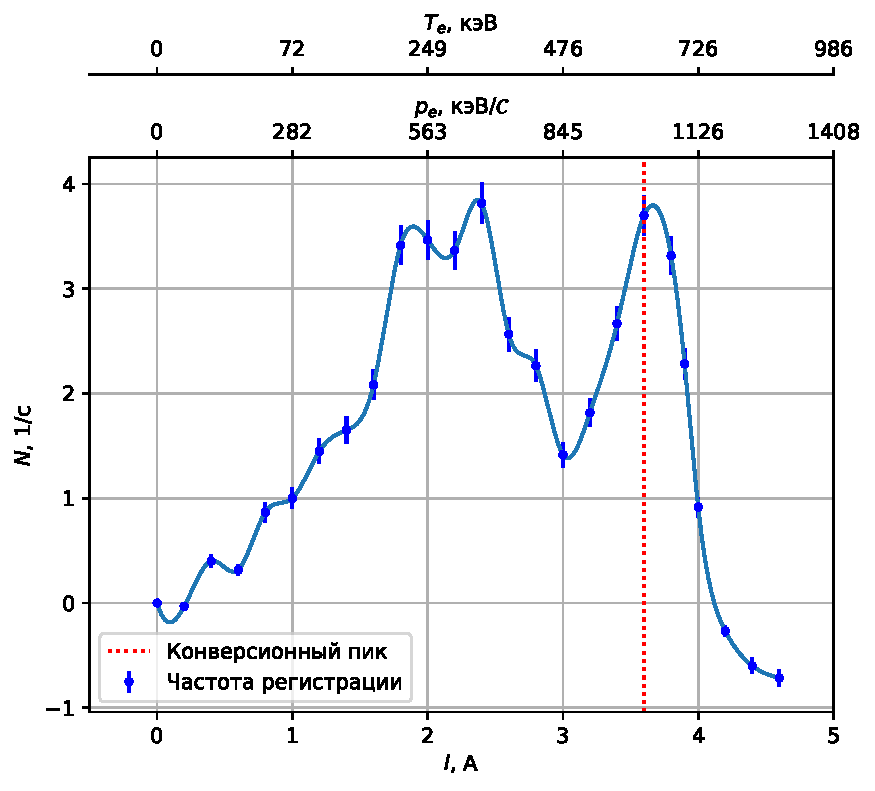
\includegraphics[width=0.8\linewidth]{gen/spectrum.pdf}
		\caption{Зависимость частоты регистрации частиц от тока.}
		\label{fig:exp_spectrum}
	\end{figure}

	На графике наблюдается конверсионный пик. Для $^{137}$Cs он расположен на $T_k = 624$ кэВ. Таким образом, нормируем график по энергии и импульсам $T_e$, $p_e$.

	Исходя из ширины конверсионного пика оценим разрешающую способность спектрометра.
	$$ \Delta p_e \approx 24 \text{ кэВ}/\mathcal{C}.$$
	
	
	% \begin{table}[h!]
	% 	\footnotesize
	% 	\begin{tabular}{cccc}
\toprule
$I$, A & $N$, 1/с & $p_e$, $\text{кэВ}/\mathcal{C}$ & $T_e$, кэВ \\
\midrule
0.00 & 1.37 & 0.00 & 0.00 \\
0.20 & 1.33 & 56.30 & 3.09 \\
0.40 & 1.77 & 112.61 & 12.26 \\
0.60 & 1.68 & 168.91 & 27.19 \\
0.80 & 2.23 & 225.21 & 47.43 \\
1.00 & 2.37 & 281.52 & 72.41 \\
1.20 & 2.81 & 337.82 & 101.57 \\
1.40 & 3.02 & 394.12 & 134.33 \\
1.60 & 3.45 & 450.43 & 170.18 \\
1.80 & 4.78 & 506.73 & 208.65 \\
2.00 & 4.83 & 563.03 & 249.35 \\
2.20 & 4.73 & 619.34 & 291.93 \\
2.40 & 5.18 & 675.64 & 336.12 \\
2.60 & 3.93 & 731.94 & 381.67 \\
2.80 & 3.63 & 788.25 & 428.39 \\
3.00 & 2.78 & 844.55 & 476.11 \\
3.20 & 3.18 & 900.85 & 524.69 \\
3.40 & 4.03 & 957.16 & 574.02 \\
3.60 & 5.06 & 1013.46 & 624.00 \\
3.80 & 4.68 & 1069.76 & 674.55 \\
3.90 & 3.65 & 1097.92 & 700.01 \\
4.00 & 2.28 & 1126.07 & 725.59 \\
4.20 & 1.10 & 1182.37 & 777.07 \\
4.40 & 0.77 & 1238.68 & 828.94 \\
4.60 & 0.65 & 1294.98 & 881.15 \\
\bottomrule
\end{tabular}

	% 	\caption{Исходные и обработанные данные эксперимента.}
	% 	\label{tab:data}
	% \end{table}

	В соответствии с \eqref{eq:fermi} построим график Ферми.
	$$ \sqrt{N(p_e)} \cdot p_e^{-3/2} \propto T_{max} - T.$$

	\begin{figure}[h!]
		\centering
		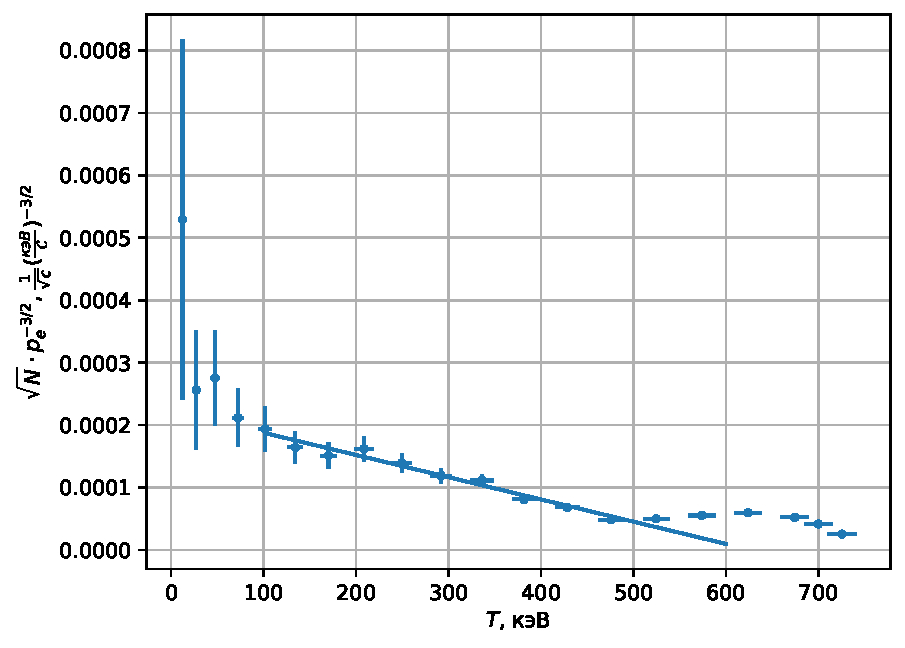
\includegraphics[width=0.7\linewidth]{gen/fermi.pdf}
		\caption{Зависимость частоты регистрации частиц от тока.}
		\label{fig:exp_fermi}
	\end{figure}
	
	На графике есть линейный участок, его экстраполяция пересекает ось абсцисс в точке $T = T_{max}$.
	
	\begin{table}[h!]
		\footnotesize
		\begin{tabular}{cccccccccc}
\toprule
$\overline{x}$ & $S_x$ & $\overline{y}$ & $S_y$ & $R_{xy}$ & r & $a$ & $\Delta a$ & $b$ & $\Delta b$ \\
\midrule
255.80 & 11280.50 & 1.32e-04 & 1.50e-09 & -4.02e-03 & -0.977050 & -3.56e-07 & 2.93e-08 & 2.23e-04 & 8.13e-06 \\
\bottomrule
\end{tabular}

		\caption{Аппроксимация линейного участка.}
		\label{tab:mnk}
	\end{table}
	
	$$T_{max} = \frac{-b}{a} = (627 \pm 62) \text{ кэВ}.$$
	
	Построим теоретическую зависимость $N(I)$ исходя из \eqref{eq:probability}.
	
	\begin{figure}[h!]
		\centering
		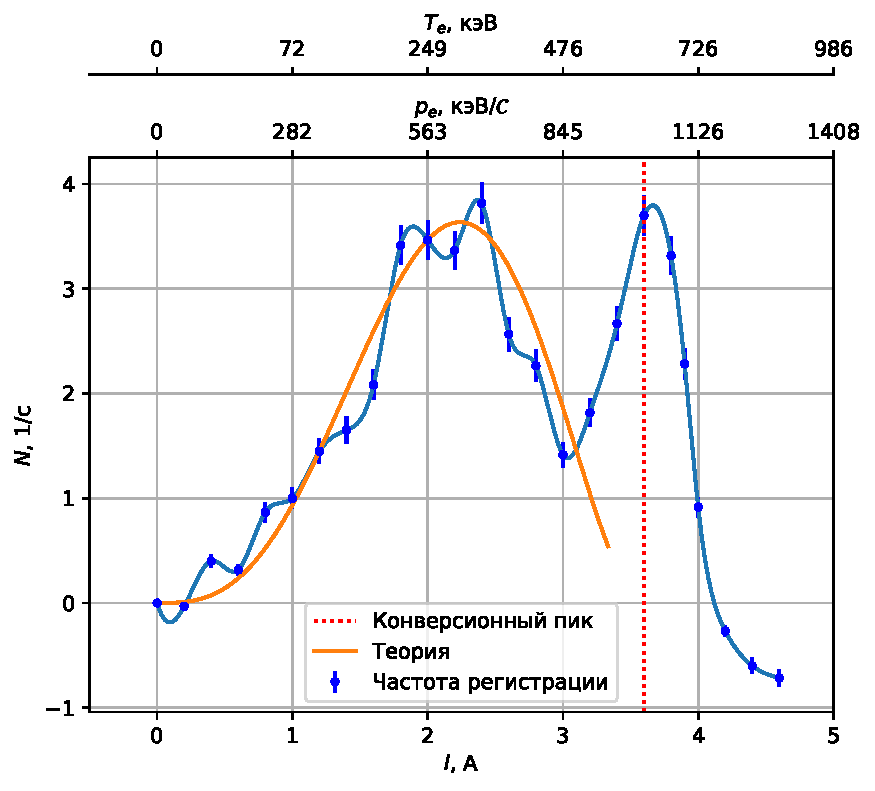
\includegraphics[width=0.7\linewidth]{gen/spectrum_fermi.pdf}
		\caption{Зависимость частоты регистрации частиц от тока.}
		\label{fig:th_spectrum}
	\end{figure}
	
	Как можно видеть, теоретическая зависимость хорошо описывает экспериментальный результат.

\newpage

\section{Заключение и выводы}
	
	В работе определено значение максимальной энергии $\beta$-частиц при распаде $^{137}$Cs $T_{max} = (627 \pm 62)$ кэВ.
	
	Подтверждена теоретическая зависимость $N(p_e)$.
	
	Определено значение разрешающей способности спектрометра $\Delta p_e \approx 24 \text{ кэВ}/{\mathcal{C}}$.
		
\end{document}








































































































































































































